\documentclass{beamer}
\usepackage{pgfpages}
\usepackage[backend=bibtex]{biblatex}
\usepackage{multicol}
\usepackage{multimedia}
\usepackage[absolute,overlay]{textpos}
\usepackage{parskip}
\usepackage{hyperref}
\usepackage{lmodern}
\usepackage{bbding}
\usepackage[absolute,overlay]{textpos}
\usepackage{framed} %Used to shade important equations, color devined with shadecolor
\usepackage{url}
\hypersetup{colorlinks=true, urlcolor=blue}
\setlength{\parskip}{\smallskipamount}
\colorlet{shadecolor}{cyan}
%\usepackage[texcoord,grid,gridunit=mm,gridcolor=red!10,subgridcolor=green!10]{eso-pic} %DELETE when done with grid
\setbeameroption{hide notes} % Only slides
%\setbeameroption{show only notes} % Only notes
%\setbeameroption{show notes on second screen=right} % Both
%\bibliography{../../papers/references.bib}
\setbeamerfont{footnote}{size=\tiny}
%\AtEveryCitekey{\clearfield{title}}

%
% Choose how your presentation looks.
%
% For more themes, color themes and font themes, see:
% http://deic.uab.es/~iblanes/beamer_gallery/index_by_theme.html
%
\mode<presentation>
{
\usetheme{Warsaw}      % or try Darmstadt, Madrid, Warsaw, ...
\usecolortheme{default} % or try albatross, beaver, crane, ...
\usefonttheme{default}  % or try serif, structurebold, ...
\setbeamertemplate{navigation symbols}{}
\setbeamertemplate{caption}[numbered]
} 

\usepackage[english]{babel}
%\usepackage[utf8x]{inputenc} %Doesn't play well with biblatex
\usepackage{amssymb}
\usepackage{bm}
\usepackage{color}
\usepackage{graphicx}
\setbeamercovered{invisible}
\setbeamercovered{%
again covered={\opaqueness<1->{100}}} %This changes the opaqueness of each bullet

\newcommand{\red}[1]{{\color{red}{#1}}}
\newcommand{\checkH}[2]{\begin{textblock*}{1cm}(#1,#2){\Huge \red{\Checkmark}}\end{textblock*}}
\newcommand{\checkh}[2]{\begin{textblock*}{1cm}(#1,#2){\huge \red{\Checkmark}}\end{textblock*}}
\newcommand{\checkL}[2]{\begin{textblock*}{1cm}(#1,#2){\Large \red{\Checkmark}}\end{textblock*}}
\newcommand{\checkl}[2]{\begin{textblock*}{1cm}(#1,#2){\large \red{\Checkmark}}\end{textblock*}}
\renewcommand{\rm}[1]{\mathrm{#1}}

\title[{\color{white}{Heat Transfer - Radiation}}]{Radiation as a Mechanism for Heat Transfer}
\author{Cody Petrie}
\institute{Southern Utah University}
\date{}

\begin{document}

%\setbeamertemplate{frametitle}[default][center]
\begin{frame}
\titlepage
\end{frame}

% Uncomment these lines for an automatically generated outline.
%\begin{frame}{Outline}
%  \tableofcontents
%\end{frame}

% Commands to include a figure:
%\begin{figure}
%\includegraphics[width=\textwidth]{your-figure's-file-name}
%\caption{\label{fig:your-figure}Caption goes here.}
%\end{figure}

\begin{frame}{Quiz}
\begin{center}
{\Large NO QUIZ TODAY}
\end{center}
I was told that that my lesson can't have any effect on your grades
\end{frame}

\begin{frame}{Questions}
\begin{center}
   Which student do you think will learn the most here?
   ~\\~\\~
   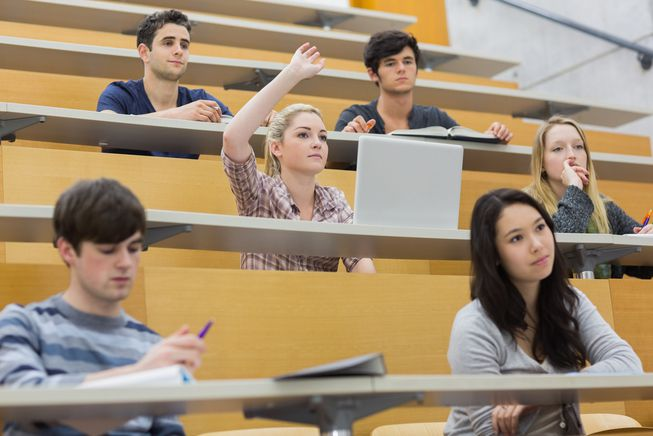
\includegraphics[width=0.9\textwidth]{figures/asking_questions.jpg}
\end{center}
\end{frame}

\begin{frame}[t]{Radiation}
What do you think of when you hear the word radiation?
\only<2->{
   \begin{textblock*}{\textwidth}(0.3cm,1.8cm) % {block width} (coords)
      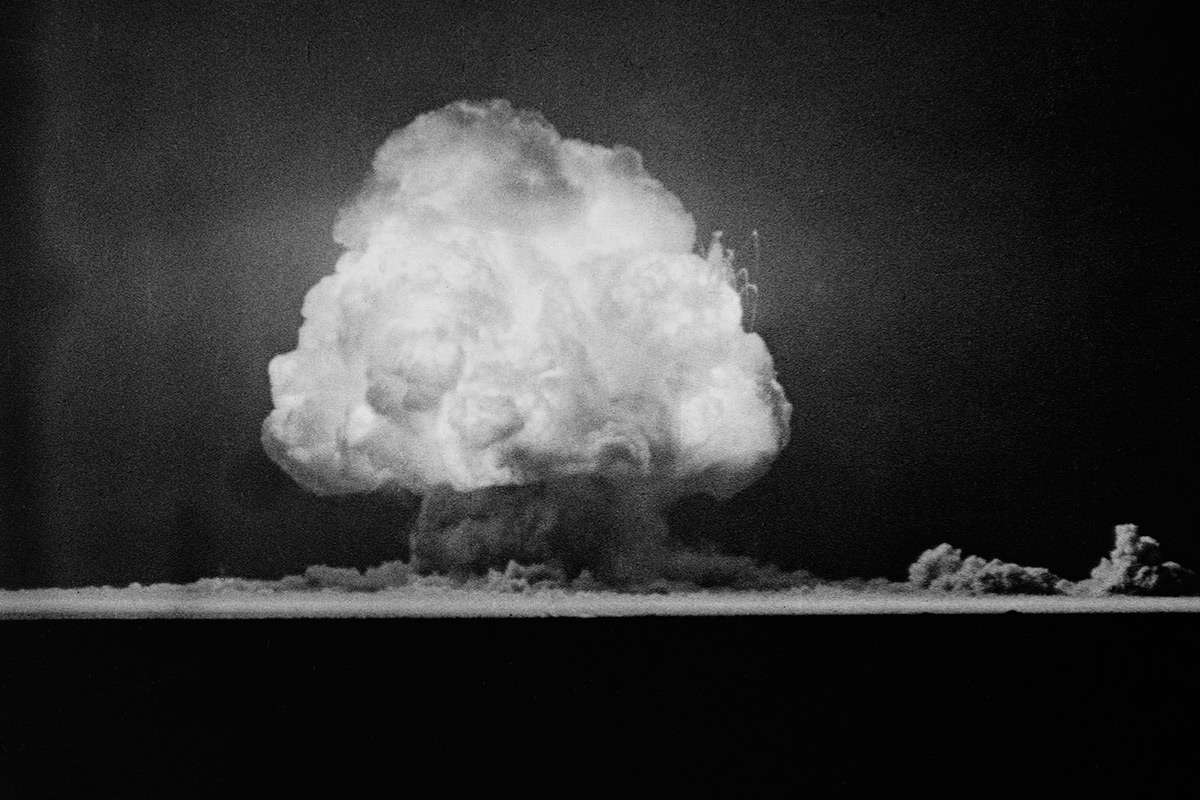
\includegraphics[width=8.0cm]{figures/trinity.jpg}
   \end{textblock*}
}
\only<3->{
   \begin{textblock*}{\textwidth}(7.5cm,2.0cm) % {block width} (coords)
      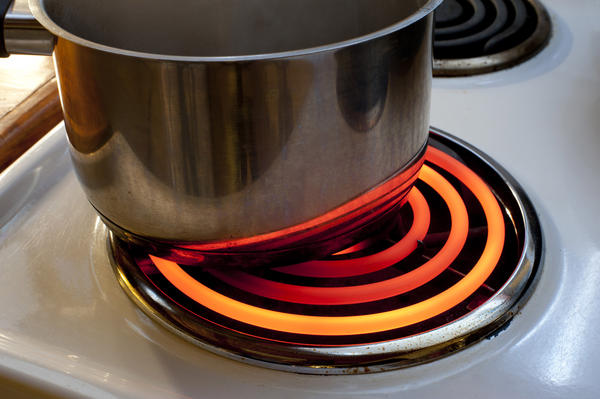
\includegraphics[width=4.5cm]{figures/pan_on_stove.jpg}
   \end{textblock*}
   \begin{textblock*}{\textwidth}(6.5cm,5.6cm) % {block width} (coords)
      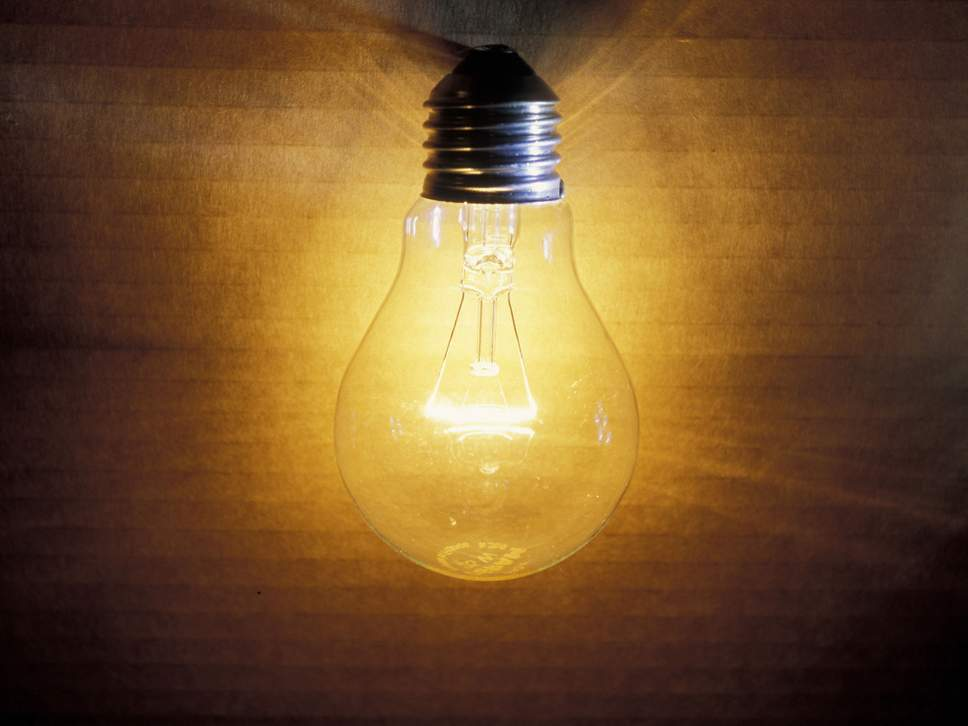
\includegraphics[width=4.5cm]{figures/light_bulb.jpg}
   \end{textblock*}
}
\only<4->{
   \begin{textblock*}{\textwidth}(2.5cm,3.0cm) % {block width} (coords)
      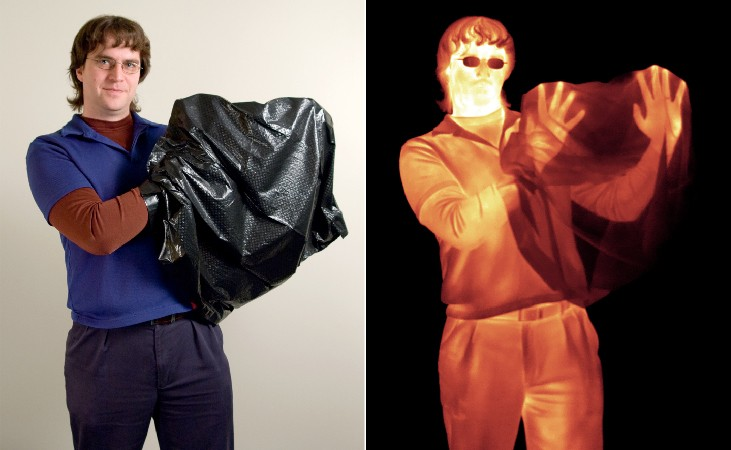
\includegraphics[height=5.0cm,trim={0 0 13cm 0},clip]{figures/infrared.jpg}
   \end{textblock*}
}
\only<5->{
   \begin{textblock*}{\textwidth}(2.5cm,3.0cm) % {block width} (coords)
      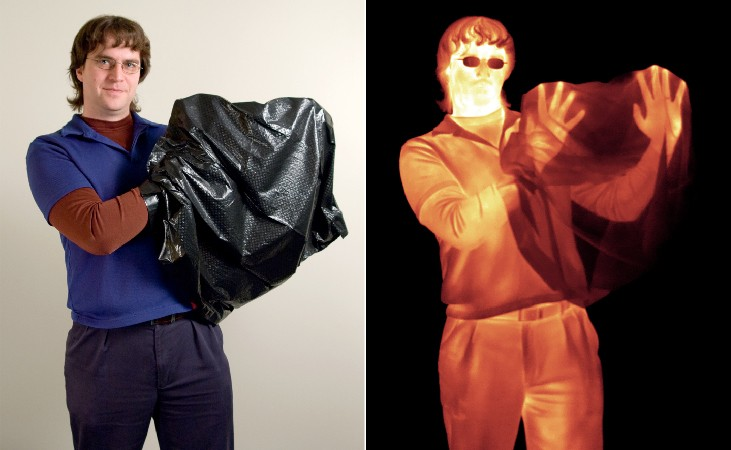
\includegraphics[height=5.0cm]{figures/infrared.jpg}
   \end{textblock*}
}
\only<6->{
   \begin{textblock*}{\textwidth}(2.0cm,2.3cm) % {block width} (coords)
      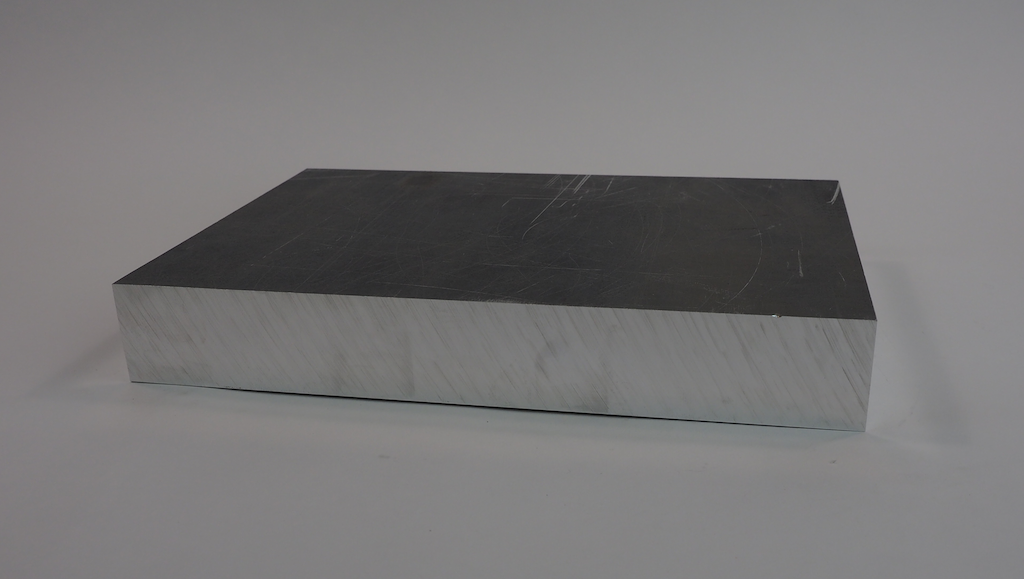
\includegraphics[width=10.0cm]{figures/metal.png}
   \end{textblock*}
}
\end{frame}

\begin{frame}[t]{Review}
\begin{itemize}
   \item<1-> What is {\bf internal energy}?
   \begin{itemize}
      \item<2-> The energy of all of the internal pieces (atoms and molecules) of an object, as seen at rest.
   \end{itemize}
   \item<3-> What about {\bf work} and {\bf heat}?
   \begin{itemize}
      \item<4-> Work is energy being transfered by some force.
      \begin{align*}
         dW&=\mathbf{F}\cdot d\mathbf{r}~~~~~~~~~~~~~~~~~~~~~~~~~~~~~~~~\\
         dW&=-PdV~~~~~~~~~~~~~~~~~~~~~~~~~~~~~~~~
      \end{align*}
      \vspace{-0.8cm}
      \item<5-> Heat is the flow of energy from one thing to \\ another, usually because of a temperature \\ difference.
   \end{itemize}
\end{itemize}
\only<2->{
   \begin{textblock*}{\textwidth}(9.5cm,3.5cm) % {block width} (coords)
      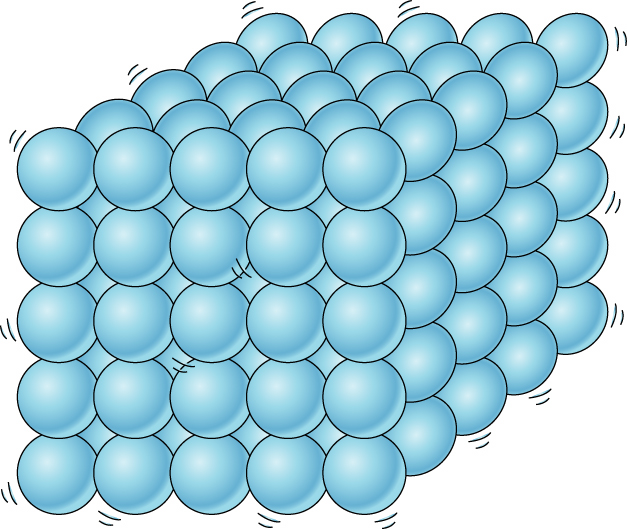
\includegraphics[width=3.0cm]{figures/vibrating_solid.jpg}
   \end{textblock*}
}
\only<4->{
   \begin{textblock*}{\textwidth}(1.0cm,6.6cm) % {block width} (coords)
      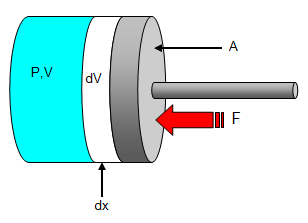
\includegraphics[width=3.0cm]{figures/work.png}
   \end{textblock*}
}
\only<5->{
   \begin{textblock*}{\textwidth}(5.0cm,6.2cm) % {block width} (coords)
      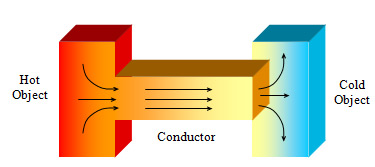
\includegraphics[width=5.0cm]{figures/heat_flow.jpg}
   \end{textblock*}
}
\end{frame}

\begin{frame}[t]{First Law of Thermodynamics}
\begin{itemize}
   \item With these three things ($E_\text{int}$, $W$, $Q$) can you remember what the first law of thermodynamics is {\bf and what it means}?
   \only<2->{
   \begin{equation*}
      \Delta E_\text{int} = Q + W
   \end{equation*}
   }
   \item<3-> Are those heat {\bf taken from} or {\bf added to}, and work {\bf done on} or {\bf done by} the system? {\it Discuss with the person next to you until you agree on something.}
   \only<4->{
   \begin{equation*}
      \Delta E_\text{int} = Q_\text{added to} + W_\text{done on}
   \end{equation*}
   }
\end{itemize}
\end{frame}

\begin{frame}[t]{Check for Understanding}
\begin{center}
   I have a gas contained in a metal cylinder with a piston. I want to temporarily raise the energy of the gas contained in the cylinder. How should I do it and how much will it change the energy by?
   \begin{textblock*}{\textwidth}(5.0cm,3.0cm) % {block width} (coords)
      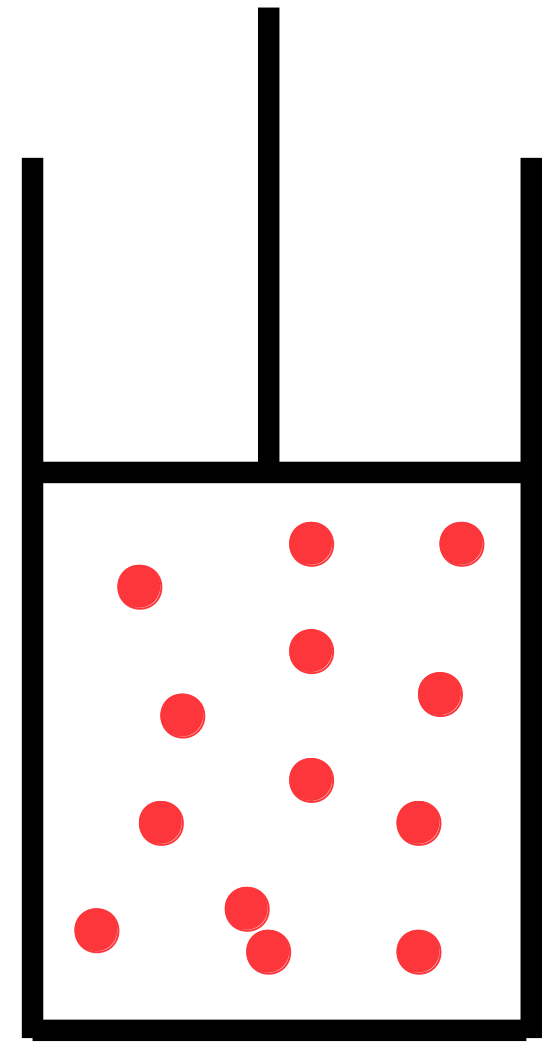
\includegraphics[width=3.0cm]{figures/mypiston.png}
   \end{textblock*}
   \begin{enumerate}[A.]
      \item Move the piston down, $\Delta E\text{int} = \int\limits_{V_i}^{V_f} PdV$
      \item Move the piston down, $\Delta E\text{int} = -\int\limits_{V_i}^{V_f} PdV$
      \item Move the piston up, $\Delta E\text{int} = \int\limits_{V_i}^{V_f} PdV$
      \item Move the piston up, $\Delta E\text{int} = -\int\limits_{V_i}^{V_f} PdV$
      \item Quit and give up
   \end{enumerate}
\only<2>{\checkl{0.5cm}{4.0cm}}
\end{center}
\end{frame}

\begin{frame}[t]{Check for Understanding - Again}
\begin{center}
   Same situation, we want to add energy, but since we used a metal cylinder the piston rusted and won't move. What should we do now to add energy? ~\\~\\~\\
   \begin{textblock*}{\textwidth}(5.0cm,3.0cm) % {block width} (coords)
      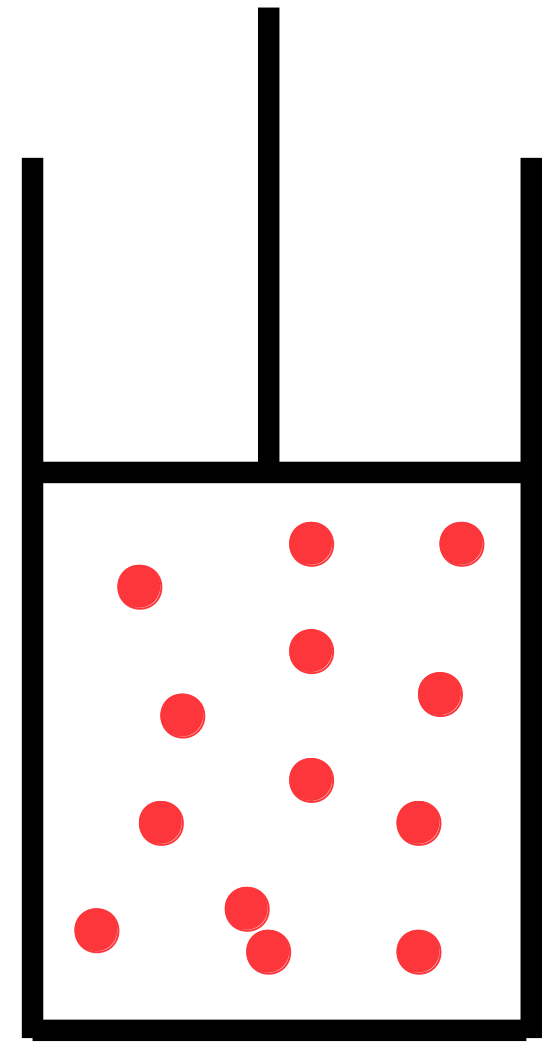
\includegraphics[width=3.0cm]{figures/mypiston.png}
   \end{textblock*}
   \begin{enumerate}[A.]
      \item Keep pushing on the piston
      \item Wait for a really long time for something to \\ happen
      \item Give up, but give the container a good hard \\ kick to make yourself feel better
   \end{enumerate}
\only<2>{\checkl{0.5cm}{4.8cm}}
\end{center}
\only<2>{\Large ~\\~\\And this leads us into our \\ next topic: heat transfer
}
\end{frame}

\begin{frame}{Mechanisms for Energy Transfer}
\begin{itemize}
   \item {\bf Conduction:} Kinetic energy is exchanged between atoms and molecules as they collide.
   \begin{center}
      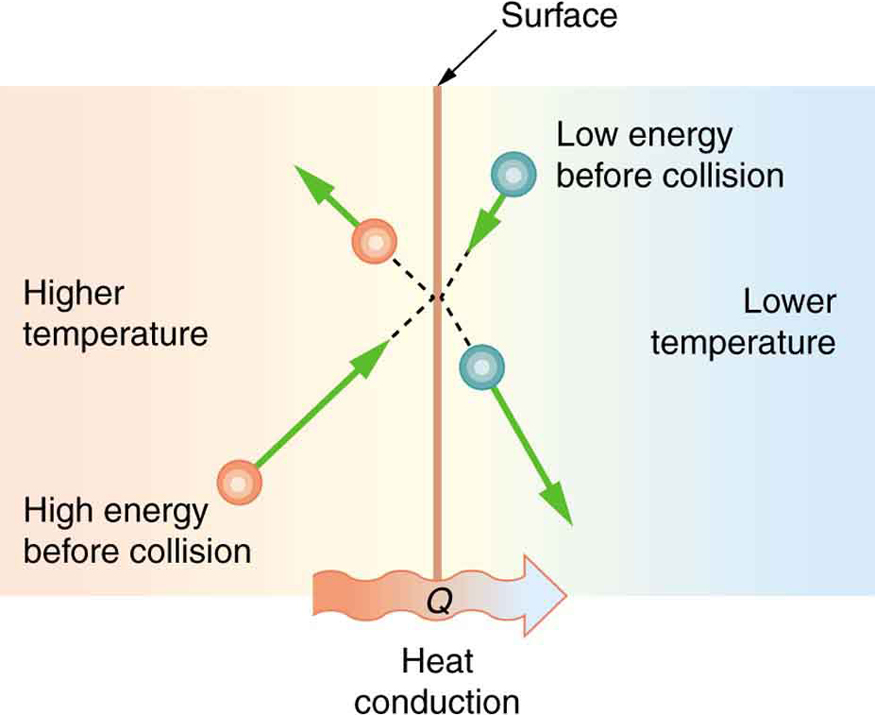
\includegraphics[height=3cm]{figures/conduction1.jpg}
      ~
      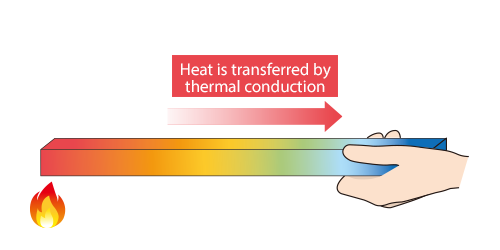
\includegraphics[height=3cm]{figures/conduction2.png}
   \end{center}
   \uncover<2>{
   \item {\bf Convection:} Some bulk medium that has some energy is moving and carrying that energy with it.
   \begin{center}
      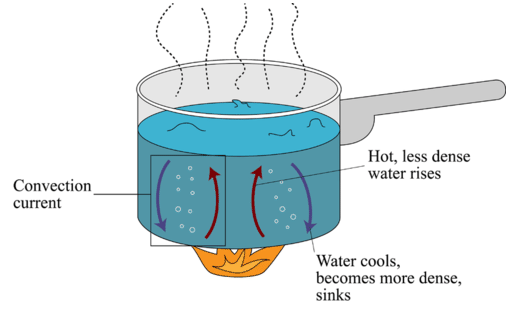
\includegraphics[height=3cm]{figures/convection.png}
   \end{center}
   }
\end{itemize}
\end{frame}

\begin{frame}[t]{Thermal Radiaton}
\begin{itemize}
   \item The third way in which an object can transfer/move energy is through {\bf radiation}.
   \item<2-> All things radiate, but only things that radiate in the visible part of the spectrum ``glow."
%\begin{center}
%   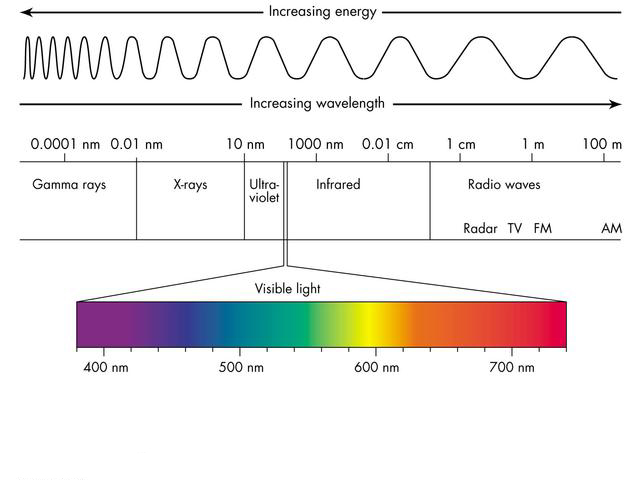
\includegraphics[width=8.0cm]{figures/EMspectrum.jpg}
%   ~ 
%   \only<2->{
%   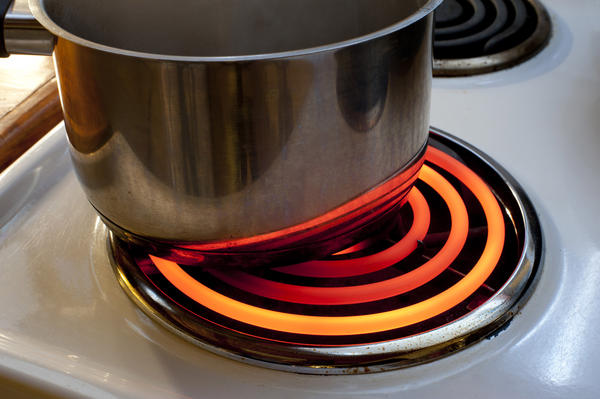
\includegraphics[width=4.5cm]{figures/pan_on_stove.jpg}
%   }
%\end{center}
\begin{textblock*}{\textwidth}(0.25cm,3.3cm) % {block width} (coords)
   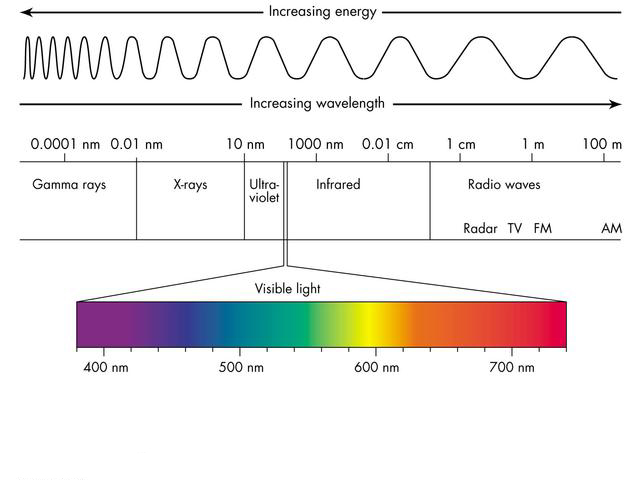
\includegraphics[width=8.0cm]{figures/EMspectrum.jpg}
\end{textblock*}
\only<2->{
\begin{textblock*}{\textwidth}(8.5cm,5.0cm) % {block width} (coords)
   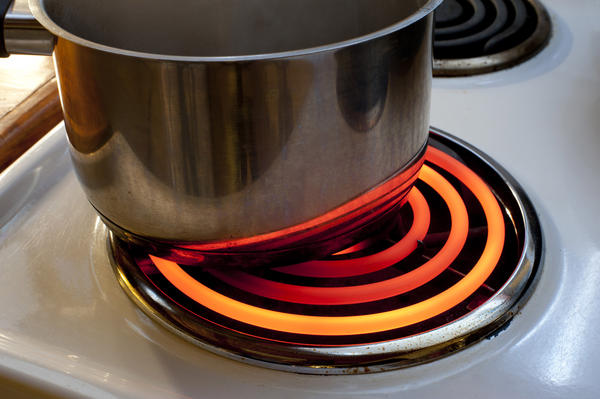
\includegraphics[width=4.5cm]{figures/pan_on_stove.jpg}
\end{textblock*}
}
\end{itemize}
\end{frame}

\begin{frame}[t]{Thermal Radiation}
\begin{itemize}
   \item Why do things radiate energy as Electromagnetic (EM) waves/radiation at all?
   \item<2-> It turns out that when charged particles change velocity they radiate energy as EM waves. The more they change their velocity the more energy they radiate.
\end{itemize}
~\\
\only<2->{
\begin{columns}
\begin{column}{0.5\textwidth}
\begin{center}
   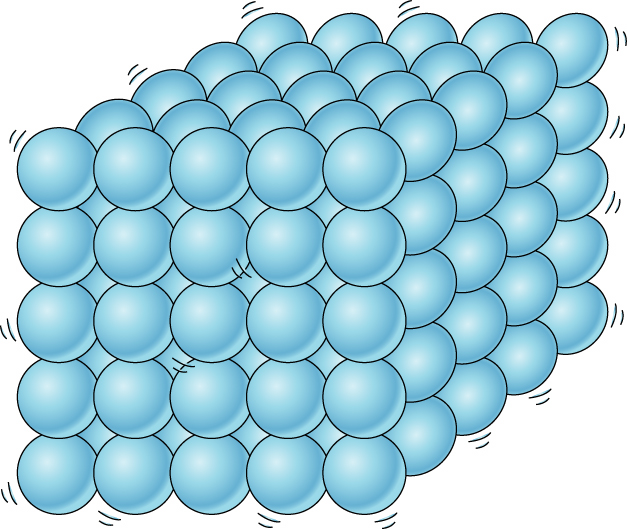
\includegraphics[width=\textwidth]{figures/vibrating_solid.jpg}
\end{center}
\end{column}
\begin{column}{0.5\textwidth}
   In fact, absorbing EM waves (radiation from other things) will cause the particles of move around more, which in turn causes them to radiate more.
\end{column}
\end{columns}
}
\end{frame}

\begin{frame}{Thermal Radiation}
\begin{itemize}
   \item But how much energy does something radiate?
   \item Question for your group: Do you think a ``hotter" object will radiate more or less {\bf and why}?
   \item<2-> In 1879 Josef Stefan studied how much power was radiated by hot platinum filaments and found that $P \propto T^4$.
\begin{center}
   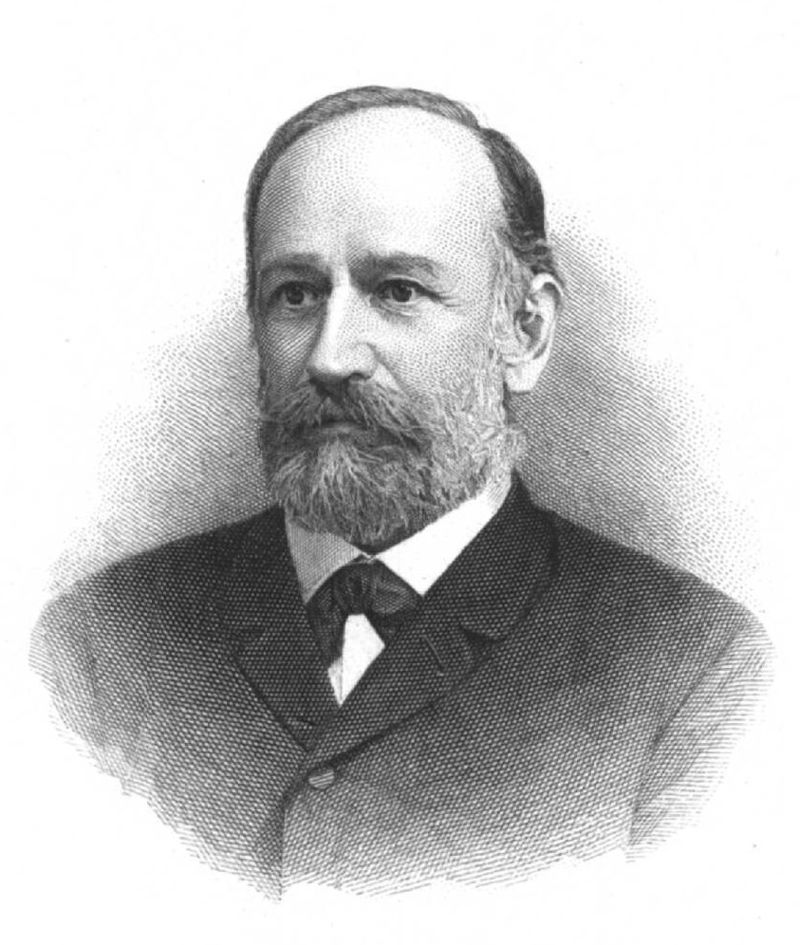
\includegraphics[width=0.20\textwidth]{figures/stefan.jpg}
   ~~~~
   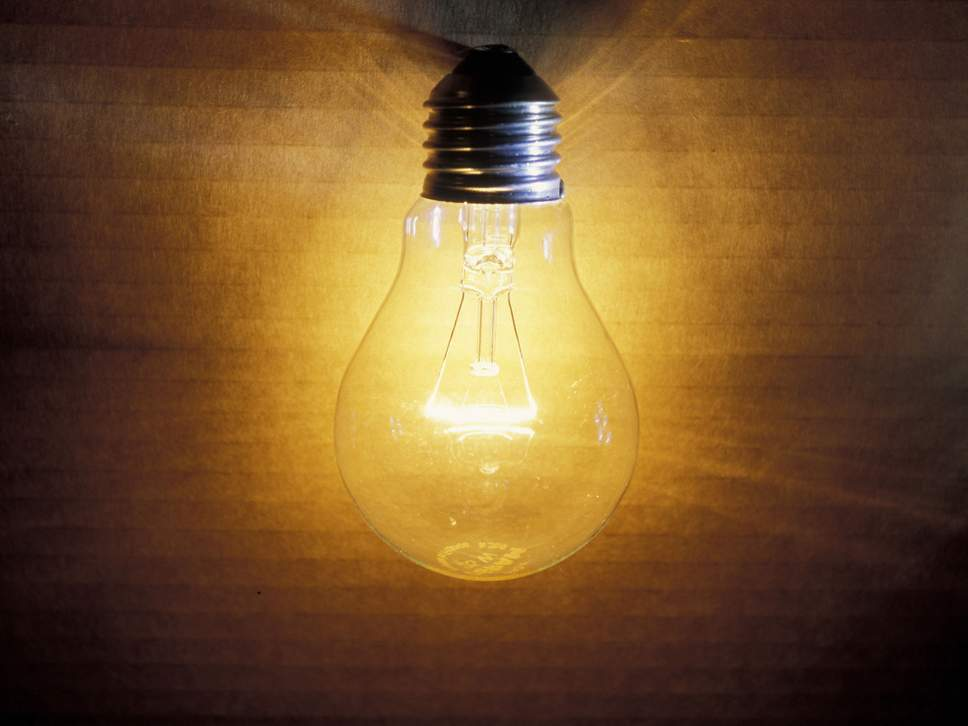
\includegraphics[width=0.30\textwidth]{figures/light_bulb.jpg}
\end{center}
\item<2-> This is what we now call the Stefan-Boltzmann Law (Boltzmann discovered the same thing a few year after Stefan)
\begin{center}
\colorbox{orange}{\parbox{0.3\textwidth}{
   \begin{eqnarray*}
      ~~~~~ P = \sigma A e T^4
   \end{eqnarray*}
}}
\end{center}
\end{itemize}
\end{frame}

\begin{frame}{Stefan-Boltzmann Law}
\begin{itemize}
   \item Let's look at each piece of this law so we know what they are.
   \begin{equation*}
      P = \sigma A e T^4
   \end{equation*}
   \item<2> \underline{$P$} is the power radiated. The power contained in the EM waves. Remember that power is energy/time so the units are Watts (Joules/sec).
   \item<3> \underline{$\sigma$} is a constant of proportionality. $\sigma = 5.6696 \times 10^{-8}$ W/m$^2\cdot$K$^4$.
   \item<4> \underline{$A$} is the objects surface area in meters$^2$. This makes sense because more ``stuff" means more things to radiate.
   \item<5> \underline{$e$} is called the {\bf emissivity} and it takes values from 0 to 1. Not all things are good at absorbing and radiating EM energy, so to account for this we experimentally determine how well things radiate, 1 being a ``perfect" radiator and 0 doesn't radiate at all.
   \item<6> \underline{$T$} is temperature in K.
\end{itemize}
\end{frame}

\begin{frame}{Emissivity, $e$}
\begin{itemize}
   \item Another name for the emissivity is the absorptivity, which is the fraction of absorbed energy to indicent energy.
   \begin{equation*}
      e = a = \frac{\text{Amount of radiation that is absorbed}}{\text{Amount of radiation that hits the surface}}
   \end{equation*}
   \item<2> If an object is good at absorbing light then it must be good at radiating it (otherwise you would get a build up of energy).
\end{itemize}
\uncover<2>{
\begin{center}
   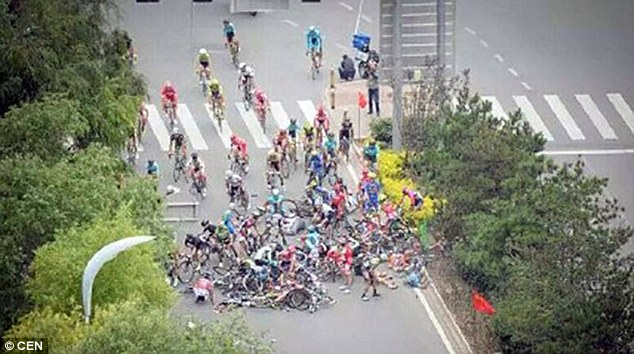
\includegraphics[width=0.70\textwidth]{figures/pileup.jpeg}
   \\ This object likes to absorb bikes but doesn't like to radiate them.
\end{center}
}
\end{frame}

\begin{frame}{Check for Understanding}
\begin{center}
   Which of these has high and which has low emissivity?
   ~\\~\\
   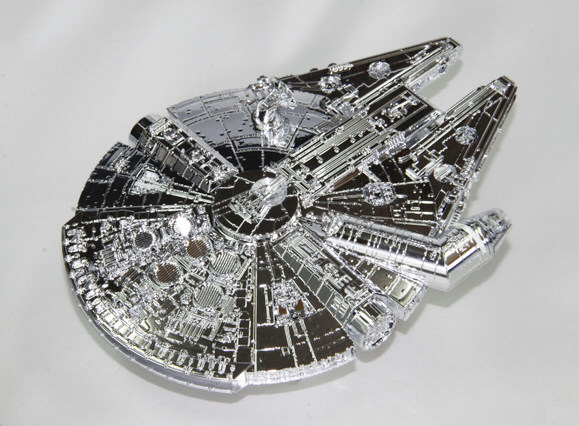
\includegraphics[width=0.40\textwidth]{figures/falcon.jpg}
   ~~~~
   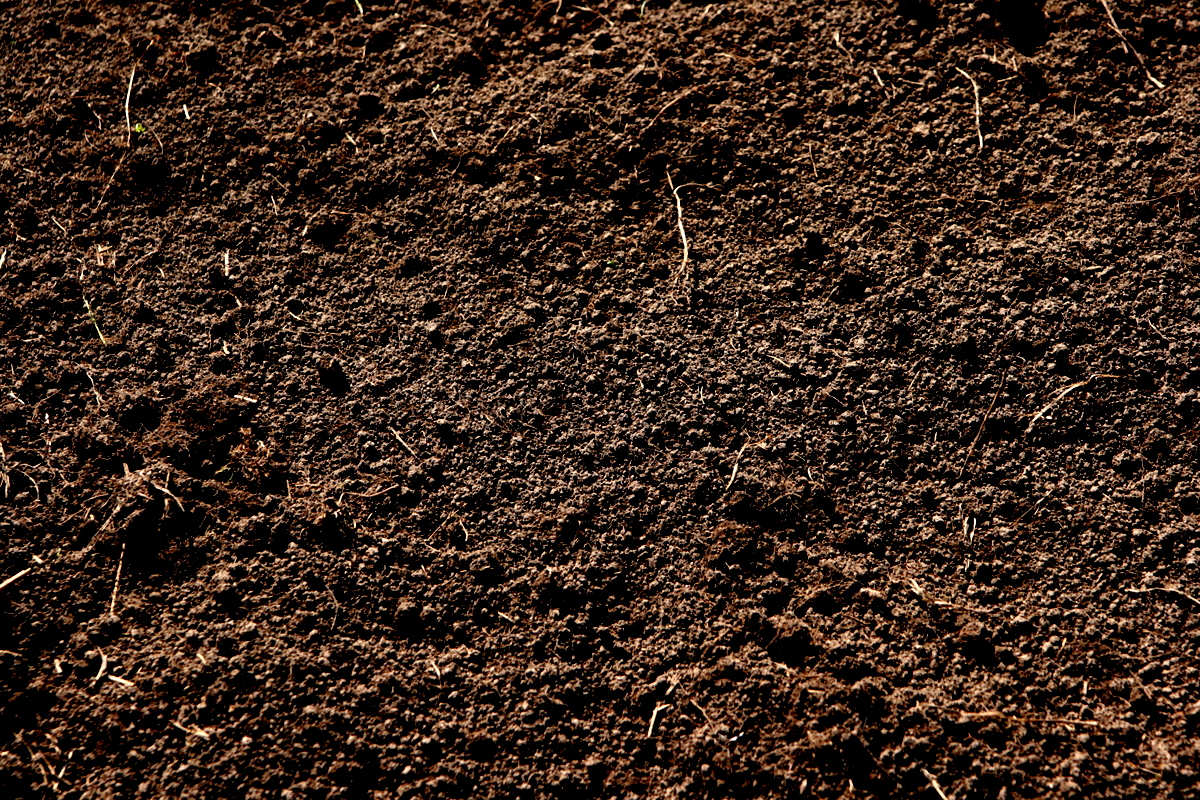
\includegraphics[width=0.40\textwidth]{figures/dirt.jpg}
   \uncover<2>{
   \\ Low ~~~~~~~~~~~~~~~~~~~~~~~~~~~~~~~~ High \\~\\
   Emissivity is how well an object absorbs EM radiation. The earth's soil has a high emmissivity of about $e=0.95$.
   }
\end{center}
\end{frame}

\begin{frame}{Check for Understanding}
Why don't things just radiate all of their energy and end up at absolute zero, i.e. $T=0$ K?
\uncover<2>{
\begin{enumerate}[A.]
   \item Nothing is allowed to be at absolute zero, so it's just not allowed.
   \item Most things prefer warmer temperatures.
   \item If things radiate they also absorb radiation.
   \item Everything is at absolute zero.
\end{enumerate}
}
\uncover<3>{
\begin{center}
   ~\\~In fact things only cool down because of radiation if they are a higher temperature than their surroundings. If $T_\text{object}=T_\text{surroundings}$ then they both radiate about the same amount and absor the same amount, so they lose and gain the same amount of energy.
   \begin{equation*}
      P_\text{net} = \sigma A e \left(T^4-T_0^4\right)
   \end{equation*}
\end{center}
}
\only<3->{\checkl{0.8cm}{3.5cm}}
\end{frame}

\begin{frame}{Check for Understanding - Cool Nights}
\begin{center}
   Why does the earth cool down at night, given
   \begin{equation*}
      P_\text{net} = \sigma A e \left(T^4-T_0^4\right)?
   \end{equation*}
   \uncover<2>{
      The earth loses energy at night because $T_0$ is the temperature of empty space but increases in temperature during the day because $T_0$ is affected by the presence of the hot sun.
   }
\end{center}
\end{frame}

\begin{frame}{Black Body}
\begin{itemize}
   \item An object that is a ``perfect" absorber (and emitter) has $e=1$ and is often called a {\bf black body}.
   \item Why the name black? Because it absorbes ALL incident light (or EM radiation).
\end{itemize}
\begin{center}
   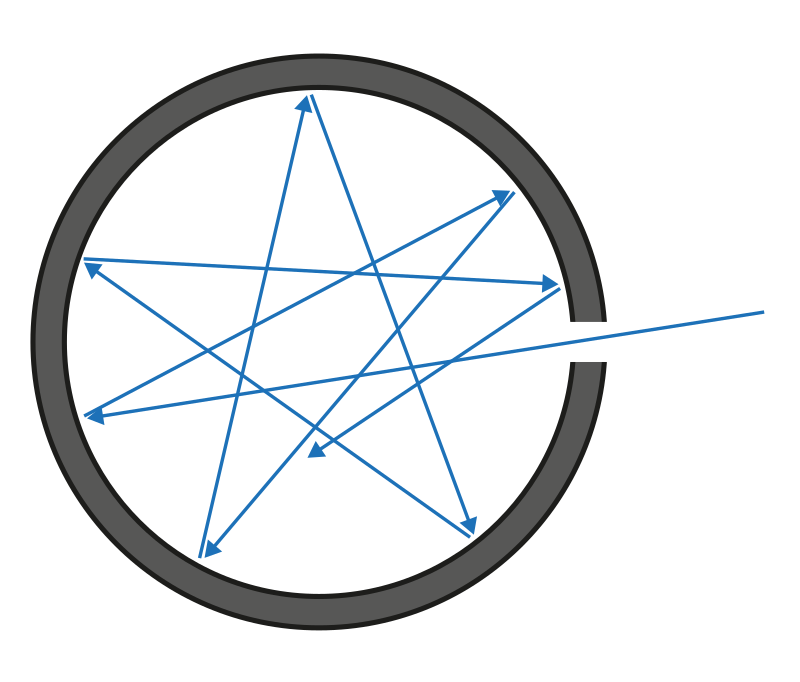
\includegraphics[width=0.40\textwidth]{figures/black_body.png}
\end{center}
\end{frame}

\begin{frame}{Examples of Black Bodies}
\begin{center}
   Nothing is exactly a black body, but some things are pretty close.
   ~\\~\\
   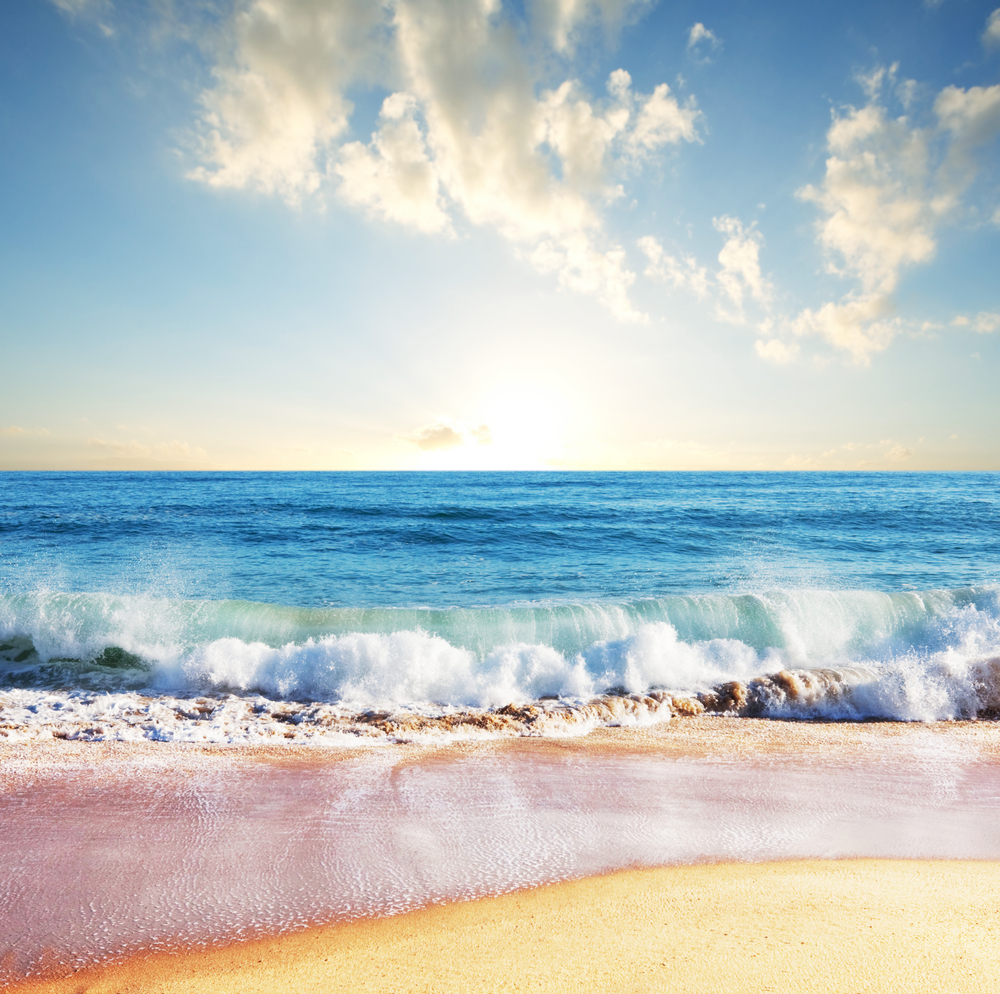
\includegraphics[width=0.25\textwidth]{figures/ocean.jpg}
   ~~~~~
   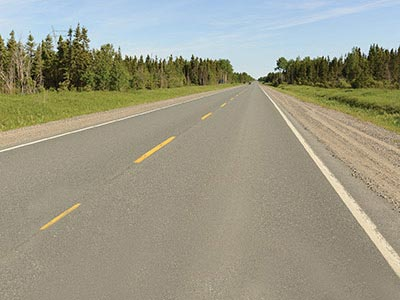
\includegraphics[width=0.35\textwidth]{figures/asphalt.jpg}
   ~~~~~
   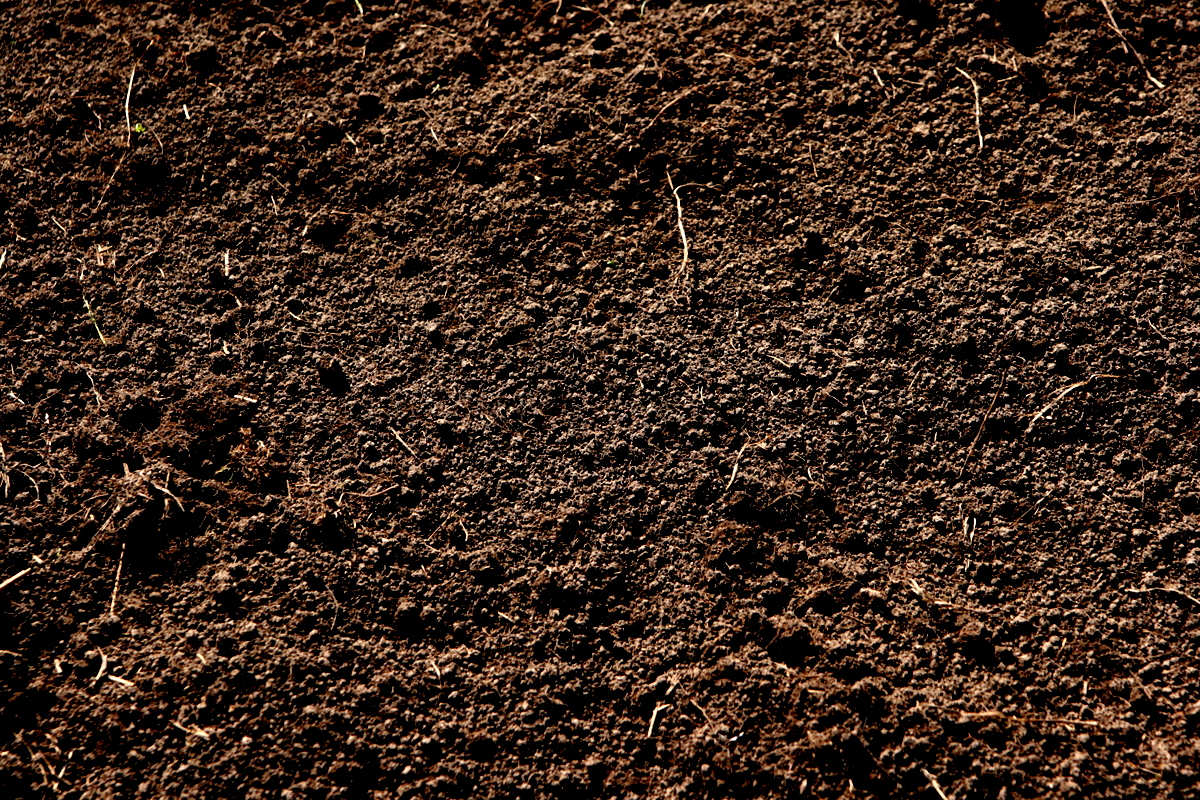
\includegraphics[width=0.35\textwidth]{figures/dirt.jpg}
   \\ $e\approx0.96$~~~~~~~~~~~~~~~~~~~~~~~$e\approx0.93$~~~~~~~~~~~~~~~~~~~~~$e\approx0.95$
   \uncover<2>{
      \\~\\ The {\bf earth} is made mostly of these things and so the earth can also be considered a black body. The {\bf sun} is also very close to being a black body
   }
\end{center}
\end{frame}

\begin{frame}[t]{Black Body Spectrum}
\begin{center}
   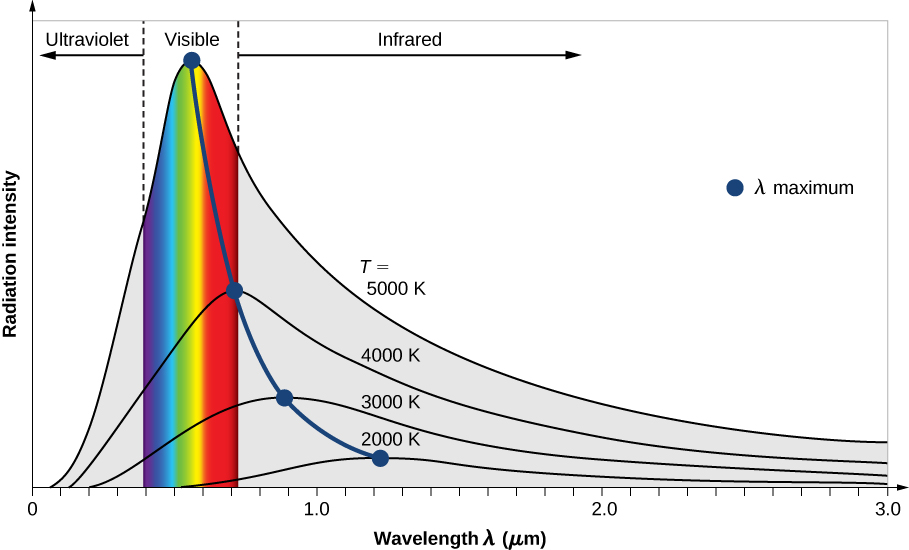
\includegraphics[width=0.8\textwidth]{figures/bb_spectrum.jpg}
\end{center}
\only<1-2>{
\begin{center}
   ~\\~
   Does the $\lambda_\text{peak}$ of radiation increase or decrease with temperature?
   ~\\~
   A.$)$ Increase ~~~~~ B.$)$ Decrease
\end{center}
}
\only<2>{\checkl{6.6cm}{7.8cm}}
\only<3-4>{
\begin{center}
   ~\\~
   Do high or low $T$ objects radiate more IR radiation?
   ~\\~
   A.$)$ High ~~~~~ B.$)$ Low
\end{center}
}
\only<4>{\checkl{4.5cm}{7.4cm}}

\end{frame}

\begin{frame}{Check for Understanding - Sun Spots}
\begin{columns}
\begin{column}{0.7\textwidth}
   Sun spots are cool places on the sun's surface that show up every 11 years. Even though they are cooler the total radiation from the sun increases when they are present. Let's model this assuming the sun takes up 10\% of the sun's surface area. Let's also assume that the sunspots are 1000K cooler than the normal surface and that the rest of the surface heats up by 90K when the sun spots are present. ~\\~
   \begin{enumerate}[A.]
      \item Calculate the output power of the sun without sun spots.
      \item Calculate the output power of the sun WITH sun spots and compare to part A. ~\\
   \end{enumerate}
   \begin{align*}
      \text{Reminder: } P = \sigma A e T^4
   \end{align*}
\end{column}
\begin{column}{0.36\textwidth}
\begin{center}
   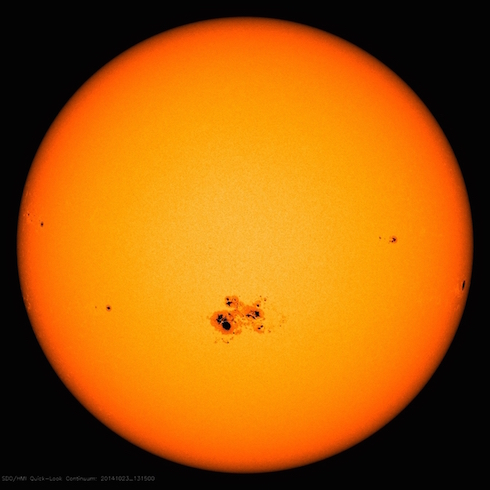
\includegraphics[width=\textwidth]{figures/sunspot.jpg}
   \\$T_\text{sun} = 5800$K
   \\$T_\text{sun spot} = 4800$K
   \\$T_\text{sun w/ spots} = 5890$K
   \\$e_\text{sun}=0.965$
   \\$A_{sun}=5.10\times10^{14}$ m$^2$
   \\$\sigma = 5.6696 \times 10^{-8}$ W/m$^2\cdot$K$^4$
\end{center}
\end{column}
\end{columns}
\end{frame}

\begin{frame}{Check for Understanding - Sun Spots}
\begin{center}
   For part A:
   \begin{align*}
      P_\text{A} &= \sigma A e T^4 \\
      &= (5.6696 \times 10^{-8}\text{ W/m}^2\text{K}^4)(5.10\times10^{14}\text{ m}^2)(0.965)(5800\text{ K})^4 \\
      &= 3.1576\times10^{22}
   \end{align*}
   For part B:
   \begin{align*}
      P_\text{B} &= \sigma (0.1 A) e T_\text{sun spot}^4 + \sigma (0.9 A) e T_\text{sun w/ spots}^4 \\
      &= (5.6696 \times 10^{-8}\text{ W/m}^2\text{K}^4)(0.1\cdot5.10\times10^{14}\text{ m}^2)(0.965)(4800\text{ K})^4 \\
      &~~+ (5.6696 \times 10^{-8}\text{ W/m}^2\text{K}^4)(0.9\cdot5.10\times10^{14}\text{ m}^2)(0.965)(5890\text{ K})^4 \\
      &= 3.1705\times10^{22}
   \end{align*}

\end{center}
\end{frame}

\begin{frame}{Check for Understanding - Project}
\begin{center}
   Using these ideas of thermal transport (conduction, convection, and radiation) design with your group the most effective thermal inculating cup that you can think of.
   \uncover<2>{
      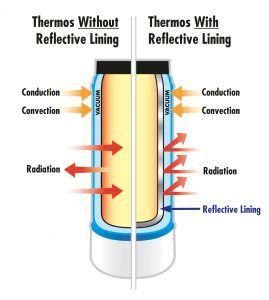
\includegraphics[width=0.5\textwidth]{figures/thermos.jpg}
   }
\end{center}
\end{frame}

\begin{frame}{Check for Understanding - Warm Cloudy Nights}
\begin{center}
   Explain why nights with cloud cover are warmer than nights with clear skies?
   \uncover<2>{
      ~\\~\\~Some of the earth's radiation gets reflected back down by the moisture in the clouds, just like the radiation trying to escape an insulated cup with a reflective coating.
   }
\end{center}
\end{frame}

\begin{frame}{Picture References}
\tiny
Student asking question, accessed 4 Mar 2019: \href{https://www.mnn.com/family/family-activities/blogs/app-lets-students-ask-questions-anonymously}{https://www.mnn.com/family/family-activities/blogs/app-lets-students-ask-questions-anonymously}
Trinity bomb, accessed 28 Feb 2019: \href{https://www.newscientist.com/article/2120748-glass-from-nuclear-test-site-shows-the-moon-was-born-dry/}{https://www.newscientist.com/article/2120748-glass-from-nuclear-test-site-shows-the-moon-was-born-dry/}\\
Pan on stove, accessed 28 Feb 2019: \href{https://stockarch.com/images/business-and-industry/energy/pan-red-hot-hotplate-8009}{https://stockarch.com/images/business-and-industry/energy/pan-red-hot-hotplate-8009}\\
Light bulb, accessed 28 Feb 2019: \href{https://www.independent.co.uk/news/science/old-fashioned-light-bulbs-could-be-set-for-comeback-after-light-recycling-breakthrough-a6806446.html}{https://www.independent.co.uk/news/science/old-fashioned-light-bulbs-could-be-set-for-comeback-after-light-recycling-breakthrough-a6806446.html}\\
Infrared man, accessed 28 Feb 2019: \href{https://courses.lumenlearning.com/astronomy/chapter/visible-light-detectors-and-instruments/}{https://courses.lumenlearning.com/astronomy/chapter/visible-light-detectors-and-instruments/}\\
Block of metal, accessed 28 Feb 2019: \href{http://beatty-robotics.com/metalbot-work-in-process/}{http://beatty-robotics.com/metalbot-work-in-process/}\\
Vibrating solid, accessed 28 Feb 2019: \href{https://chemstuff.co.uk/academic-work/year-7/particle-model-of-solids-liquids-and-gases/}{https://chemstuff.co.uk/academic-work/year-7/particle-model-of-solids-liquids-and-gases/}
Piston, accessed 28 Feb 2019: \href{http://www.schoolphysics.co.uk/age16-19/Thermal\%20physics/Thermodynamics/text/Work_done_by_an_ideal_gas/index.html}{http://www.schoolphysics.co.uk/age16-19/Thermal\%20physics/Thermodynamics/text/Work\_done\_by\_an\_ideal\_gas/index.html}\\
Heat flow, accessed 28 Feb 2019: \href{http://www.ecd.com/support/learning-center/resources/heat-flow-happens.aspx?Post=3899\&tabid=371}{http://www.ecd.com/support/learning-center/resources/heat-flow-happens.aspx?Post=3899\&tabid=371}\\
Conduction collision, accessed 1 Mar 2019: \href{https://3c1703fe8d.site.internapcdn.net/newman/gfx/news/hires/2014/whatisheatco.jpg}{https://3c1703fe8d.site.internapcdn.net/newman/gfx/news/hires/2014/whatisheatco.jpg}\\
Conduction with hand, accessed 1 Mar 2019: \href{https://www.cradle-cfd.com/glossary/detail/0000000054?c=en}{https://www.cradle-cfd.com/glossary/detail/0000000054?c=en}\\
Convection, accessed 1 Mar 2019: \href{https://www.ck12.org/physics/convection/lesson/Convection-MS-PS/}{https://www.ck12.org/physics/convection/lesson/Convection-MS-PS/}
EM spectrum, accessed 1 Mar 2019: \href{https://sites.google.com/a/coe.edu/principles-of-structural-chemistry/relationship-between-light-and-matter/electromagnetic-spectrum}{https://sites.google.com/a/coe.edu/principles-of-structural-chemistry/relationship-between-light-and-matter/electromagnetic-spectrum}\\
Picture of Stefan, accessed 1 Mar 2019: \href{https://en.wikipedia.org/wiki/Josef_Stefan}{https://en.wikipedia.org/wiki/Josef\_Stefan}\\
Bike pileup, accessed 1 Mar 2019: \href{https://www.dailymail.co.uk/news/peoplesdaily/article-3695800/Cycle-race-ends-chaos-spectator-crosses-road-WORST-possible-moment.html}{https://www.dailymail.co.uk/news/peoplesdaily/article-3695800/Cycle-race-ends-chaos-spectator-crosses-road-WORST-possible-moment.html}\\
Millenium Falcon, accessed 1 Mar 2019: \href{https://reggiocomics.wordpress.com/2010/07/21/wf-2010-limited-x-wing-tie-fighter-millennium-falcon-chrome-plated-ver/}{https://reggiocomics.wordpress.com/2010/07/21/wf-2010-limited-x-wing-tie-fighter-millennium-falcon-chrome-plated-ver/}\\
Earth's soil, accessed 1 Mar 2019: \href{https://naturesabundance.wordpress.com/2012/05/02/composting_free_natural_fertilizer/soil-not-dirt/}{https://naturesabundance.wordpress.com/2012/05/02/composting\_free\_natural\_fertilizer/soil-not-dirt/}\\
Black body pinhole, accessed 1 Mar 2019: \href{https://en.wikipedia.org/wiki/Black_body}{https://en.wikipedia.org/wiki/Black\_body}\\
Ocean, accessed 1 Mar 2019: \href{https://www.livescience.com/32139-why-are-oceans-salty.html}{https://www.livescience.com/32139-why-are-oceans-salty.html}\\
\end{frame}

\begin{frame}{Picture References}
\tiny
Road, accessed 1 Mar 2019: \href{https://www.livescience.com/32139-why-are-oceans-salty.html}{https://www.livescience.com/32139-why-are-oceans-salty.html}\\
Black body spectrum, accessed 4 Mar 2019: \href{https://phys.libretexts.org/Bookshelves/University_Physics/Book\%3A_University_Physics_(OpenStax)/Map\%3A_University_Physics_III_-_Optics_and_Modern_Physics_(OpenStax)/6\%3A_Photons_and_Matter_Waves/6.1\%3A_Blackbody_Radiation}{https://phys.libretexts.org/Bookshelves/University\_Physics/Book\%3A\_University\_Physics\_(OpenStax)/Map\%3A\_University\_Physics\_III\_-\_Optics\_and\_Modern\_Physics\_(OpenStax)/6\%3A\_Photons\_and\_Matter\_Waves/6.1\%3A\_Blackbody\_Radiation}
Sun spots, accessed 1 Mar 2019: \href{https://spaceplace.nasa.gov/sunspot-cookies/en/}{https://spaceplace.nasa.gov/sunspot-cookies/en/}\\
Thermos, accessed 1 Mar 2019: \href{https://www.reflectixinc.com/applications/shipping-products-oem/oem-mailers/how-does-it-work/}{https://www.reflectixinc.com/applications/shipping-products-oem/oem-mailers/how-does-it-work/}\\
\end{frame}

\end{document}
